\documentclass[
    DIV=12,
    cleardouble=plain,
    headings=normal,
    pdftex,
    %headexclude,footexclude,
    final
]{scrreprt}

%\usepackage{spreadtab}
\usepackage{xspace}
\usepackage[ngerman]{babel}
\usepackage[utf8]{inputenc}
%\usepackage[T1]{fontenc}
\usepackage[pdftex]{graphicx}
\usepackage[bookmarks]{hyperref}
%\usepackage{scrpage2} %old
\usepackage{scrlayer-scrpage}
\usepackage{longtable}
\usepackage{caption}
%\usepackage{pgfplots} not used?
\usepackage{float}
\usepackage{xcolor}
\usepackage{color tbl}
\usepackage{tabularx}
\usepackage{multirow} % tabelle
\usepackage{listings} % code aus datei einbinden
\usepackage{scrhack}
\usepackage{comment}
\usepackage{hyperref}
% \usepackage{minted} % package for swift
\usepackage{enumerate}

% Swift language definition
\lstdefinelanguage{swift}
{
  morekeywords={
    func,if,then,else,for,in,while,do,switch,case,default,where,break,continue,fallthrough,return,
    typealias,struct,class,enum,protocol,var,func,let,get,set,willSet,didSet,inout,init,deinit,extension,
    subscript,prefix,operator,infix,postfix,precedence,associativity,left,right,none,convenience,dynamic,
    final,lazy,mutating,nonmutating,optional,override,required,static,unowned,safe,weak,internal,
    private,public,is,as,self,unsafe,dynamicType,true,false,nil,Type,Protocol,
  },
  morecomment=[l]{//}, % l is for line comment
  morecomment=[s]{/*}{*/}, % s is for start and end delimiter
  morestring=[b]" % defines that strings are enclosed in double quotes
}

\definecolor{keyword}{HTML}{BA2CA3}
\definecolor{string}{HTML}{D12F1B}
\definecolor{comment}{HTML}{008400}

\lstset{
  language=swift,
  basicstyle=\ttfamily,
  showstringspaces=false, % lets spaces in strings appear as real spaces
  columns=fixed,
  keepspaces=true,
  keywordstyle=\color{keyword},
  stringstyle=\color{string},
  commentstyle=\color{comment},
}

% word wrap with a red arrow
\lstset{
  basicstyle=\ttfamily,
  columns=fullflexible,
  frame=single,
  breaklines=true,
  postbreak=\mbox{\textcolor{red}{$\hookrightarrow$}\space},
}

\graphicspath{{./}{./images/}}

% #################################################################

%\begin{document}

\hyphenation{Cha-otn-gsch-werl}
\setlength\headheight{1.75cm}

%\ihead*{\small{Fortgeschrittene Programmierung unter SWIFT (FWPM)}}
\ohead*{
\includegraphics[height=0.05\textheight]{fh_logo}}
\pagestyle{scrheadings}

\begin{document}


\ohead*{
\includegraphics[height=0.05\textheight]{fh_logo}}
\ifoot*{\small{The Teachify Project}}
\ofoot*{\small{Prof. Dr. Sven Rill}}



\setcounter{secnumdepth}{5}
\setcounter{tocdepth}{5}
\renewcommand{\arraystretch}{1}

\parskip0.5\baselineskip plus 0.125\baselineskip minus 0.25\baselineskip
\parindent0em

\automark*[section]{chapter}

\titlehead{\begin{center}
\includegraphics[width=5cm]{fh_logo}\end{center}}
 \title{
  Teachify - Lernspiele für Kinder \\[1em]
  Dokumentation, Spezifikation, Konstruktion
}


\author{Angelina Scheler, Bastian Kusserow, Christian Pfeiffer,\\ Christian Pöhlmann, \href{mailto:jofranz90@gmail.com?subject=Swift-Studienarbeit}{Johannes Franz}, Marcel Hagmann, Maximilian Sonntag,\\Normen Krug, Patrick Niepel,
Phillipp Dümleim, Carl Phillipp Knoblauch}

\date{09.07.2018\\ Vorgelegt bei Prof. Dr. Sven Rill} %##Abgabedatum einfügen


\maketitle
\pagenumbering{roman}
\tableofcontents

%\listoftables

\newpage
\pagenumbering{arabic}

%hier die einzelnen Punkte einfügen
\chapter{Pflichtenheft}
Christian Pfeiffer, Normen Krug \& \href{mailto:jofranz90@gmail.com?subject=Swift-Studienarbeit}{Johannes Franz}


\section{Zielbestimmung}
Es ist eine Lernspiel Software für Grundschulschüler zu entwickeln, welche auf iPads ab iOS Version 10 lauffähig ist. Schüler sollen Lernspiele bzw. Aufgaben bearbeiten können, welche von den Lehrern vorher generiert werden. Nach den Spielen können Schüler ihre eigenen Leistungen ansehen. Auch Lehrer sollen einen Überblick über die Leistungen der eigenen Schüler haben. Die Ausarbeitung der App ist auf ein Semester beschränkt, das bedeutet es stehen 3 Monate zur Umsetzung zur Verfügung. Kurz vor der Abgabe ist die Funktionsfähigkeit der Software durch Tests zu bestätigen.

\subsection{Musskriterien}

\subsubsection{Allgemein}
\begin{enumerate}[a)]
\item Die App muss auf iPads mit iOS 11 laufen
\end{enumerate}



\subsubsection{Login}
\begin{enumerate}[a)]
\item Login für den Schüler
\item Login für den Lehrer
\end{enumerate}

\subsubsection{Schüler}
\begin{enumerate}[a)]
\item Übersicht über alle freigegebenen Spiele (Spiele von der Schnittstelle abrufen)
\item Übersicht über erreichte Punktzahlen
\item Spielbeschreibung anzeigen
\item Spiel spielen
\item Ergebnisse anzeigen
\item Ergebnisse über die Schnittstelle hochladen
\end{enumerate}

\subsubsection{Lehrer}
\begin{enumerate}[a)]
\item Übersicht über alle registrierten Schüler
\item Einladen von Schülern in “Klassen”
\item Anzeigen von Ergebnissen einzelner Schüler
\item Aufgaben erstellen
\end{enumerate}


\subsubsection{Schnittstelle}
\begin{enumerate}[a)]
\item Abrufen der freigegebenen Spiele für einen Schüler
\item Schüler zu Aufgaben einladen (durch den Lehrer)
\item Abspeichern der Ergebnisse der gelösten Aufgaben
\item Abrufen der Ergebnisse der gelösten Aufgaben (Lehrer)
\end{enumerate}


\subsection{Wunschkriterien}
\subsubsection{Allgemein}
\begin{enumerate}[a)]
\item Die App kann auch auf anderen iOS Geräten (iPhone) laufen
\end{enumerate}

\subsubsection{Login}
\begin{enumerate}[a)]
\item Alternative Login Methode für den Lehrer
\end{enumerate}

\subsubsection{Schüler}
\begin{enumerate}[a)]
\item Übersicht über die vergangen Spiele
\item Lösen von Aufgaben unter Zeitdruck
\item Kindgerechte und einfache Menügestaltung
\item Schüler soll es ermöglicht werden in eigenen Tempo lernen
\end{enumerate}

\subsubsection{Lehrer}
\begin{enumerate}[a)]
\item Einteilung der Schüler in Klassen
\item Ranking der Spielergebnisse der Klassen
\item Individuelle Förderung von Schülern
\end{enumerate}


\subsubsection{Schnittstelle}
\begin{enumerate}[a)]
\item Detailliertes Speichern der Spiele für eine Auswertung (gebrauchte Antwortzeit, Statistiken für Klassen)
\item Abspeichern von Bildern
\end{enumerate}


\subsection{Abgrenzungskriterien}
Das System besitzt keine Schnittstellen zu anderen Produkten.
Es existiert keine automatische Erfassung von Benutzern aus Fremddaten.

\section{Produkteinsatz}
Die App soll als Referenz für die Lehre der Fortgeschrittenen Swift 4 Entwicklung des Mobile Computing Studiengangs an der Hochschule Hof dienen.\\
\\
Hypothetisch soll die App im Rahmen des Grundschulunterrichts eingesetzt werden. Hierbei hat jeder Schüler ein eigenes Tablet und kann mit diesem Aufgaben bearbeiten. Der Lehrer kann den Schülern Aufgaben zuweisen und die Aufgaben Ergebnisse einsehen.  

\subsection{Anwendungsbereiche}
Primär Grundschulen, später Erweiterung für höhere Bildungseinrichtungen denkbar. 

\subsection{Zielgruppen}
Schüler / Studenten und Lehrer bzw. Lehrbeauftragte

\subsection{Betriebsbedingungen}
Um die App in allen Funktionen nutzen zu können, wird ein iPad mit iOS 10 mit Internetverbindung vorausgesetzt. Beim Einloggen als Schüler müssen alle freigeschalteten und geteilten Aufgaben abgerufen werden. Eingeloggte Lehrer sollen eine Übersicht über die verfügbaren Aufgabentypen sowie Schüler bzw. deren Klassen haben. Die Pflege der Schnittstelle soll Wartungsfrei sein. Die administrative Gewalt (Zuweisung der Aufgaben, sowie Einblick in die Statistik der Schüler) soll bei den Lehrern stehen.



\section{Produktfunktionen}
\subsection{/F0010/ Einloggen}
Ein beliebiger App Nutzer kann sich über den Startscreen einloggen. 
Als Kennung wird sein iCloud Account verwendet. Die App muss zwischen Schülerbenutzern und Lehrerbenutzern unterscheiden können. Die Unterscheidung dieser zwei Benutzergruppen geschieht durch unterschiedliche Loginverfahren (Zum Login eines Lehrers muss ein Button gedrückt werden,  bzw. ein QR Code verwendet werden).Nach dem Login wird der Benutzer in das seiner Benutzergruppe zugehörige Hauptmenü weitergeleitet (Schüler bzw. Lehrer).


\subsection{/F0020/ Verfügbare Spiele herunterladen (Schüler/Schnittstelle)}
Schülerbenutzer kann im Schülerhauptmenü seine ihm freigegebenen Aufgaben bzw. Spiele einsehen. Das Herunterladen dieser geschieht automatisch nach dem Login. Falls dem Schüler keine Aufgaben freigegeben wurden, wird ihm anstatt der Aufgaben ein Hinweis angezeigt.


\subsection{/F0030/ Spielinformationen anzeigen (Schüler)}
Wählt der Schüler ein ihm freigegebenes Spiel in dem Schülerhauptmenü aus, so werden ihm Informationen über das ausgewählte Spiel (Spielregeln, Schwierigkeit… etc. angezeigt).\\
Über einen ''Spiel starten'' Button, kann der Schüler das Spiel starten. Mit einer Geste bzw. einem Zurückbutton kann er zurück in das Hauptmenü gelangen.


\subsection{/F0040/ Spiel spielen (Schüler)}
Wählt der Schüler den “Spiel starten” Button in den Spielinformationen aus, wird das Spiel gestartet und  er kann die Aufgaben bearbeiten. Nach dem Bearbeiten der Aufgaben werden die Spielergebnisse über die Schnittstelle wieder hochgeladen.



\subsection{/F0050/ Leistungen anzeigen (Schüler)}
Wählt ein Schüler den ''Erfolge Tab'' in dem Schülerhauptmenü aus, so kann er seine Spielerfolge einsehen. Hierbei wird ihm eine Punktzahl, welche die Summe der innerhalb der Lernspiele erreichten Punkte ist. Zudem kann er sich eine Übersicht über seine letzten Spiele und die darin richtig bzw. falsch gelösten Aufgaben anzeigen lassen.

\subsection{/F0060/ Schüler in Klassen einladen (Lehrer/Schnittstelle/Schüler)}
Bevor der Lehrer Aufgaben verteilen kann muss er seine Schüler in eine Klasse einladen. Wenn die Schüler die Einladung der Lehrer annehmen, werden sie der Klasse hinzugefügt.

\subsection{/F0070/ Aufgaben Klassen zuteilen}
Ein Lehrer kann an einzelne Schüler spezielle Aufgaben stellen.

\subsection{/F0080/ Ergebnisse einzelner Schüler anzeigen}
Für den Lehrer muss es möglich sein, die Ergebnisse der Schüler einzusehen.

\chapter{Schüler UI, Anbindung an die Schnittstelle und Entwicklung des Mathe Piano Spiels}
Christian Pfeiffer, Normen Krug \& \href{mailto:jofranz90@gmail.com?subject=Swift-Studienarbeit}{Johannes Franz}


\section{Einleitung}
In diesem Abschnitt werden die Ziele und die Motivation des Projektes definiert. Dabei werden unter anderem die Erwartungen an das Projekt genannt.

\subsection{Motivation}
Die Hauptmotivation des Projektes war das Lernen und Einarbeiten in neue Apple Frameworks (wie \textit{SpriteKit} und \textit{CloudKit}) und Erfahrungen sammeln in der Zusammenarbeit mit mehreren Entwicklerteams, welche gleichzeitig an einem Projekt arbeiten. Deshalb war es zwingend notwendig, sich mit anderen Teams zu verständigen und auszutauschen.  

\subsection{Ziele}
Als Ziele der Studienarbeit wurden folgende Punkte definiert: 
\begin{itemize}
\item Kinderfreundliches Design und Layout
\item Erstellen eines Mathelernspieles 
\item Aufgaben die von Lehrern erstellt werden anzeigen und in ein spielbare Form überführen
\item Die von Schüler beantworteten Fragen an den Lehrer weiterleiten
\item Den Schülern die Möglichkeit bieten die Spiele im Endlos Modus, unabhängig der von Lehrer zugewiesenen Aufgaben, zu spielen
\item Lernen eines neuen Apple Frameworks (\textit{SpriteKit})
\item Erfahrung sammeln in Zusammenarbeit mit anderen Teams
\end{itemize}
\section{Spezifikation}
Als Strategie für die Umsetzung des Projektes wurde das Prinzip "Funktionalität vor UI-Design" gewählt. Als die Funktionalität dann zufriedenstellend.

\subsection{Mathe Piano Spiel}
Bei der Entwicklung des Spiels war es wichtig, möglichst schnell einen funktionsfähigen Prototypen zu ertstellen. Dieser wurde im Verlauf des Projektes immer weiter verbessert.


\subsubsection{Game Engine}
Als Grundlage wurde die von Apple entwickelte Game Engine namens \textit{SpriteKit} verwenden. Diese Engine hat einige Vorteile gegenüber anderen Spielengines:
\begin{itemize}
\item Gute Dokumentation
\item Wiederverwendungen bereits gelernter Paradigmen    
\item Einfache Integrationsmöglichkeit in die App
\item Einfache Anbindung an andere iOS API‘s
\item Swift als Programmiersprache 
\item Schnelles Entwickeln und Testen von Funktionen durch Swift Playgrounds
\end{itemize}

\subsubsection{Herausforderungen}
Nach der ausgiebigen Einarbeitung in das \textit{SpriteKit} \textit{Framework} haben sich einige Hürden ergeben. Das Verwenden von dynamischen Buttons ist nicht trivial, weil es keine Buttons per Default gibt. Deshalb muss eine eigene Button Klasse implementiert und mit der gewünschten Funktionalität erweitert werden. Des Weiteren war es schwierig den Code sinnvoll zu strukturieren, aufgrund der durch Spiel vorgegebenen skriptartigen Programmierung. %todo: hier könnte doch der Code für einen Button als Beispiel in die Doku kommen. Eher besser in der Implementierungsphase
\subsubsection{Testen des Spieles}
Um das Spiel sinnvoll und schon währendes Entwicklungsprozesses testen zu können, musste ein Generator entwickelt werden der zufällige Aufgaben generiert. Dieser befindet sich in der \textit{RandomQuestionGenerator.swift} Klasse. 
\subsubsection{Anbindungen an interne Schnittstellen}
Von Anfang an musste darauf geachtet werden das, dass Spiel an die interne Schnittstelle angebunden werden muss, die von einem anderen Team entwickelt wurde. Da die Schnittstelle nicht von Beginn an verfügbar ist, muss eine temporäre Datenstruktur implementiert werden. Diese soll einfach austauschbar und erweiterbar sein.
\subsubsection{User Interface}
Bei der Gestaltung des User Interfaces muss explizit darauf geachtet werden, dass die Software primär von Kinder bedient wird. Das bedeutet, dass die Größe der Bedienelemente deutlich größer ausfallen muss als bei herkömmlichen Applikationen.   

\section{Implementierungsphase}
An dieser Stelle wird die Implementierung der Aufgaben beschrieben. Dabei wird auf die Schnittstellenanbindung, das Mathe Piano Spiels sowie das User Interface eingegangen.
\subsection{Mathe Piano Spiel}
%normen

%todo: replace with a real example
\lstinputlisting[language=swift]{source/test.swift}


\subsection{User Interface}
\begin{figure}[H]
	\centering
  \frame{ 
  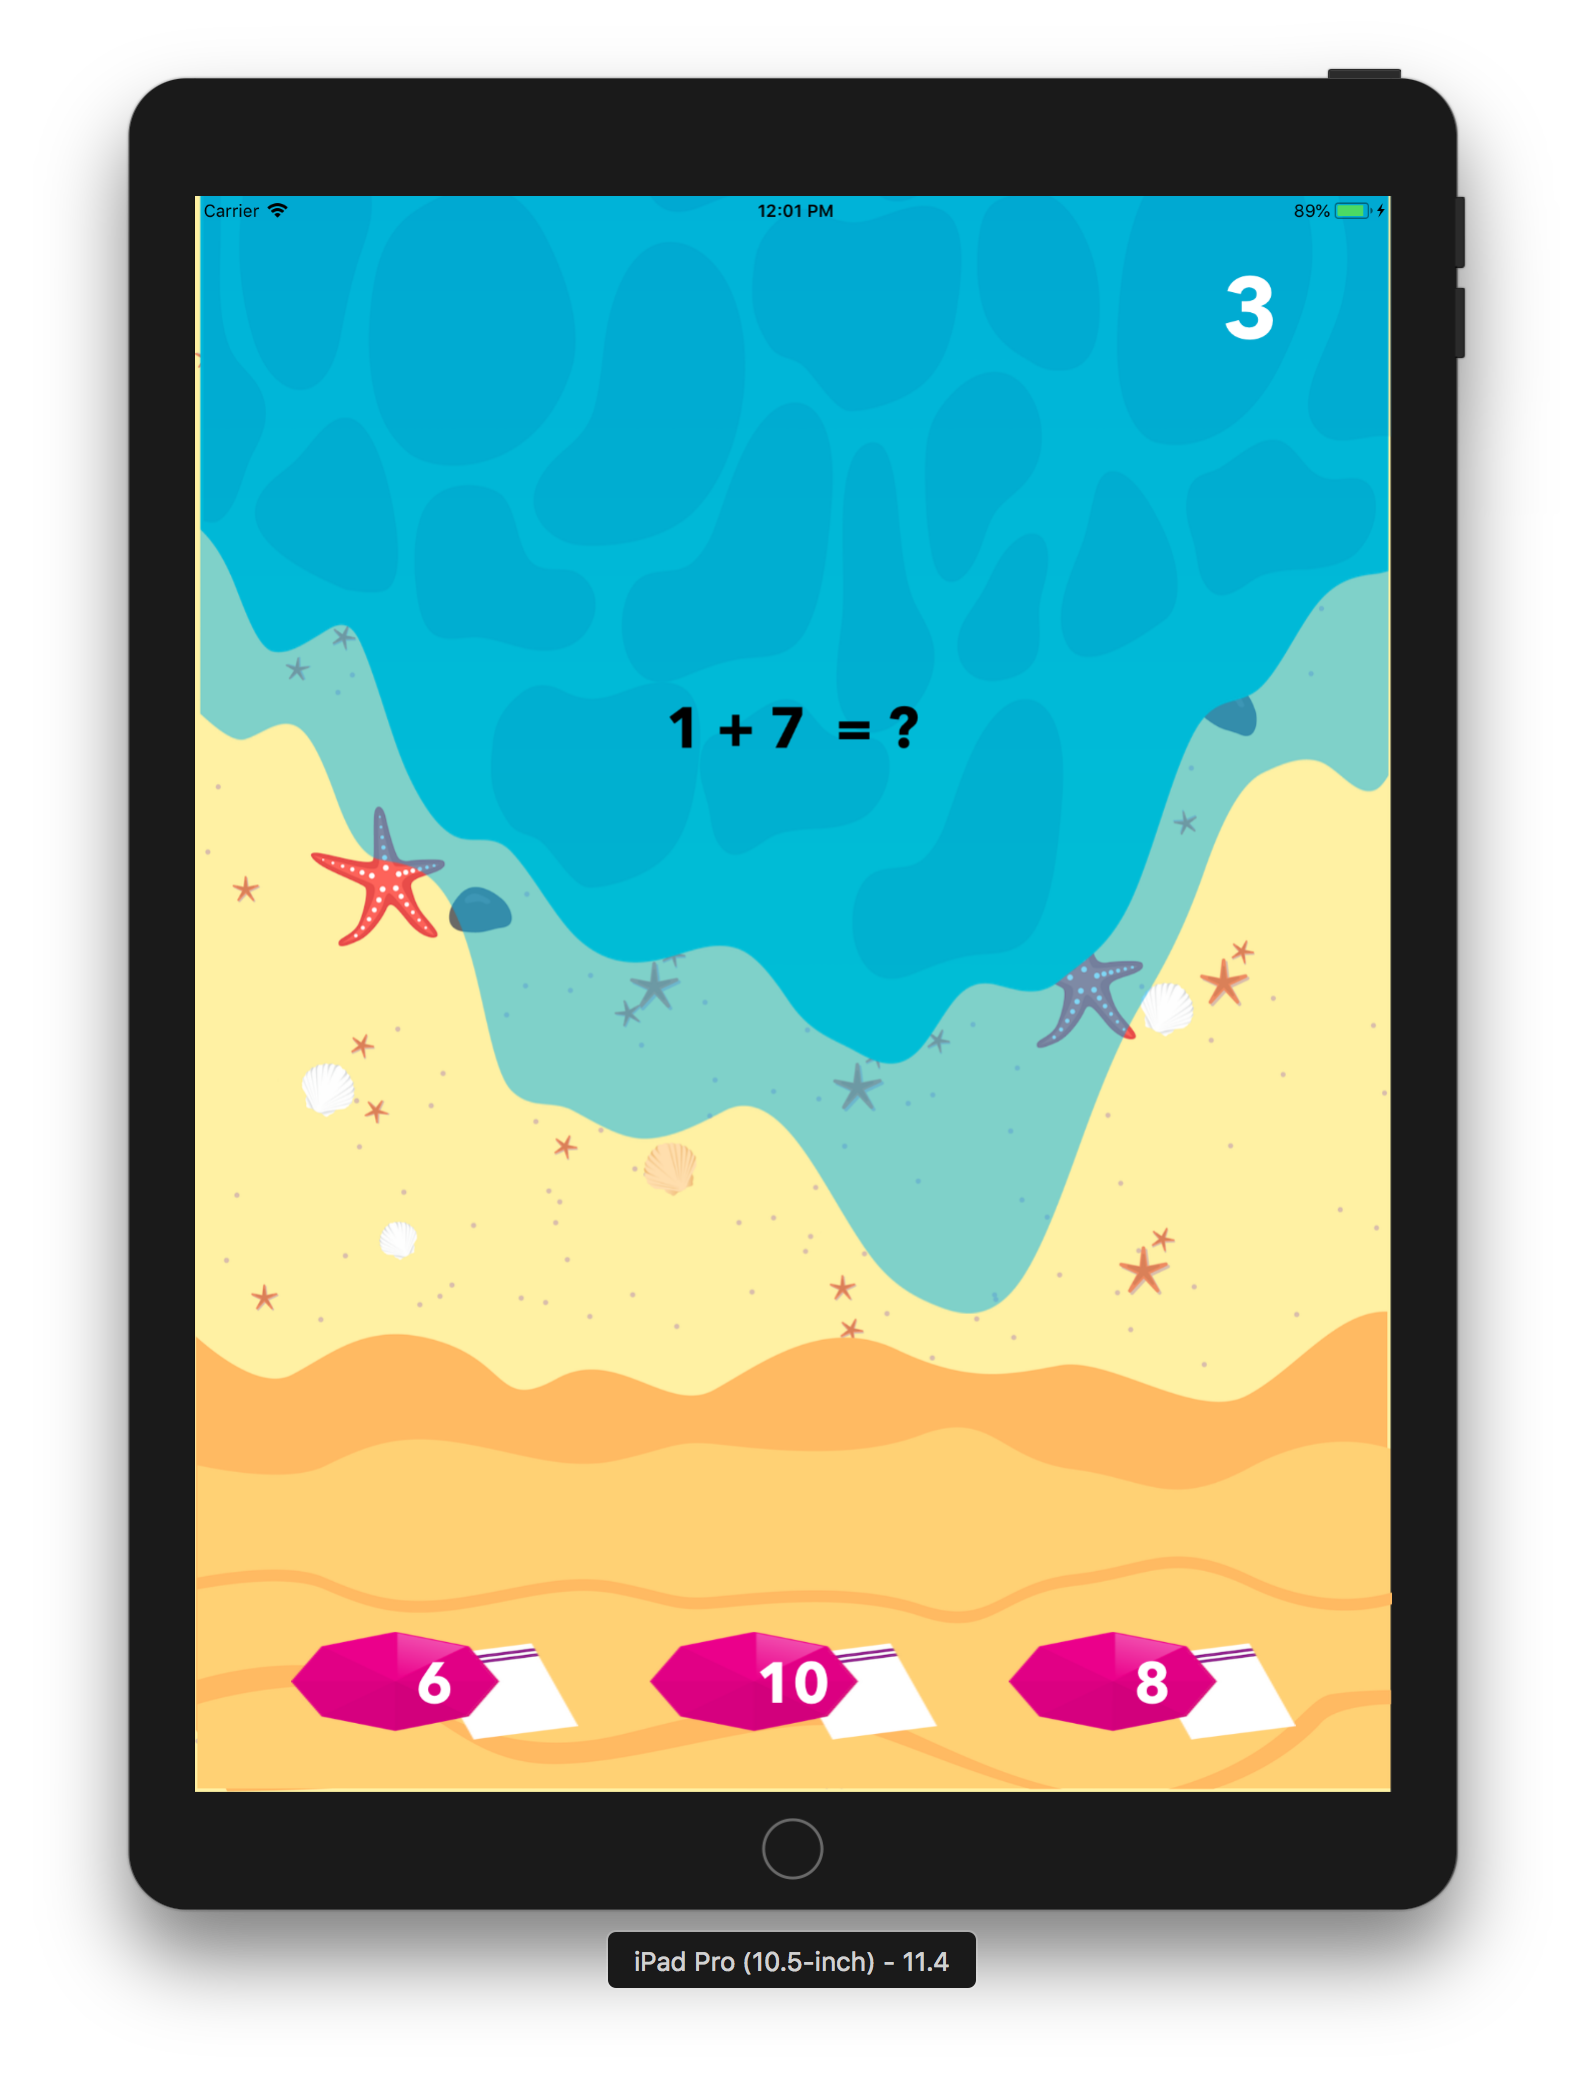
\includegraphics[width=0.5\textwidth]{images/mathPianoGame.png}
  }
	\caption{Das Mathe Piano Spiel}
	\label{Das Mathe Piano Spiel}
\end{figure}
Um das Mathepianospiel so Zielgruppen freundlich wie möglich zu gestalten, wurden verschiedene Grafiken entwickelt, welche ein typisches Strandszenario abbilden. Bei der Farbwahl wurden helle freundliche Farbtöne gewählt. Inhalt des Spiels ist eine Welle, in welcher eine Matheaufgabe abgebildet ist. Der Spieler muss die richtige Antwort auf die Matheaufgabe auswählen, bevor die Welle zu nahe kommt und die Badesachen weg spült.



\section{Fazit}
Teachify war ein herausforderendes Projekt für das 6. Semester. Dies stellte das ganze Team immer wieder vor anspruchsvolle Aufgaben. Der Umgang mit Git (\href{https://github.com/cpfeiffer3008/Teachify}{Teachify Projekt Link}) brachte zugleich viele Vorteile aber auch Herausforderungen.\\
Durch die unterschiedlichen Herangehensweisen (Design vs. Funktion) und den damit weitgehend einhergehenden Verzicht auf einen Prototypen lenkte das Projekt gegen Ende des Projektzeitraums auf einen ``Big-Bang`` Ansatz.
Positiv zu erwähnen war das Zusammenwachsen des Teams und die Zusammenarbeit untereinander. So hatten die meisten Teams eine Domäne in die sie sich eingearbeitet hatten und mussten bei der Überschneidung ihrer Gebiete zusammenarbeiten.

\section{Umsetzung des Schülerhauptmenüs \& Loginmenü}
\chapter{Implementierung eines gemeinsamen Datenmodells (TKFetchController/TKFetchSingleton \& FetchOperations)}
Bastian Kusserow (Team Lehrer) \& Christian Pfeiffer (Team Schüler)
\section{Ziele}


\begin{itemize}
\item Vermeidung von Redundanz
\item Wiederverwendbarkeit von Code
\item Ressourcenschonendes Speichern von heruntergeladenen Schnittstellendaten
\item Vereinheitlichter Zugriff und Downloadabwicklung (Fetch) von Schnittstellendaten
\end{itemize}

\section{Implementierung}

\subsection{TKModelSingleton}
Um das Ziel des Vereinheitlichten Zugriffs auf Schnittstellendaten zu erfüllen, wird eine Singleton Klasse zum Abspeichern der Schnittstellendaten verwendet.

\lstinputlisting[language=swift]{source/fetchsingleton.swift}

\subsection{TKFetchController}

\lstinputlisting[language=swift]{source/fetchsingleton.swift}

\subsection{TKFetchController - Zugriffschicht}

\lstinputlisting[language=swift]{source/fetchctrlextension.swift}

\chapter{Schüler Game Teachbird}
Christian Pöhlamnn

\section{Grundlage}
Grundlegende Information.
\chapter{Schnittstelle iCloud}
Patrick Niepel, Marcel Hagmann, Carl Philipp Knoblauch

\section{Einleitung}
In diesem Abschnitt wird die Schnittstelle mit iCloud beschrieben. Dabei wird erklärt wie die Architektur aufgebaut ist, wie mit der Schnittstelle kommuniziert wird und welche Probleme aufgetreten sind. 

\section{Warum iCloud/CloudKit?}

Wenn man bei der Entwicklung einer iOS App auf Cloud Services zurückgreifen will, bietet sich natürlich das Apple eigene CloudKit für iCloud an. Es ergab sich dadurch auch die Möglichkeit eine neues Framework kennenzulernen, da wir zuvor noch nicht mit CloudKit gearbeitet hatten. 
Über die Cloud-Schnittstelle sollen zwischen Lehrer und Schüler alle Aufgaben geteilt werden. Der Lehrer kann seine Aufgaben/Spiele in iCloud laden und diese mit seinen Schülern teilen. Die Schüler sollen dann diese Aufgaben/Spiele erledigen und ihre Lösungen wieder in iCloud laden. Dadurch wird dem Lehrer wiederum ermöglicht sich einen Überblick über die Lösungen seiner Klasse zu machen. Mit CloudKit konnten wir diese Ziele alle umsetzten.

\section{Architektur}


\begin{figure}
  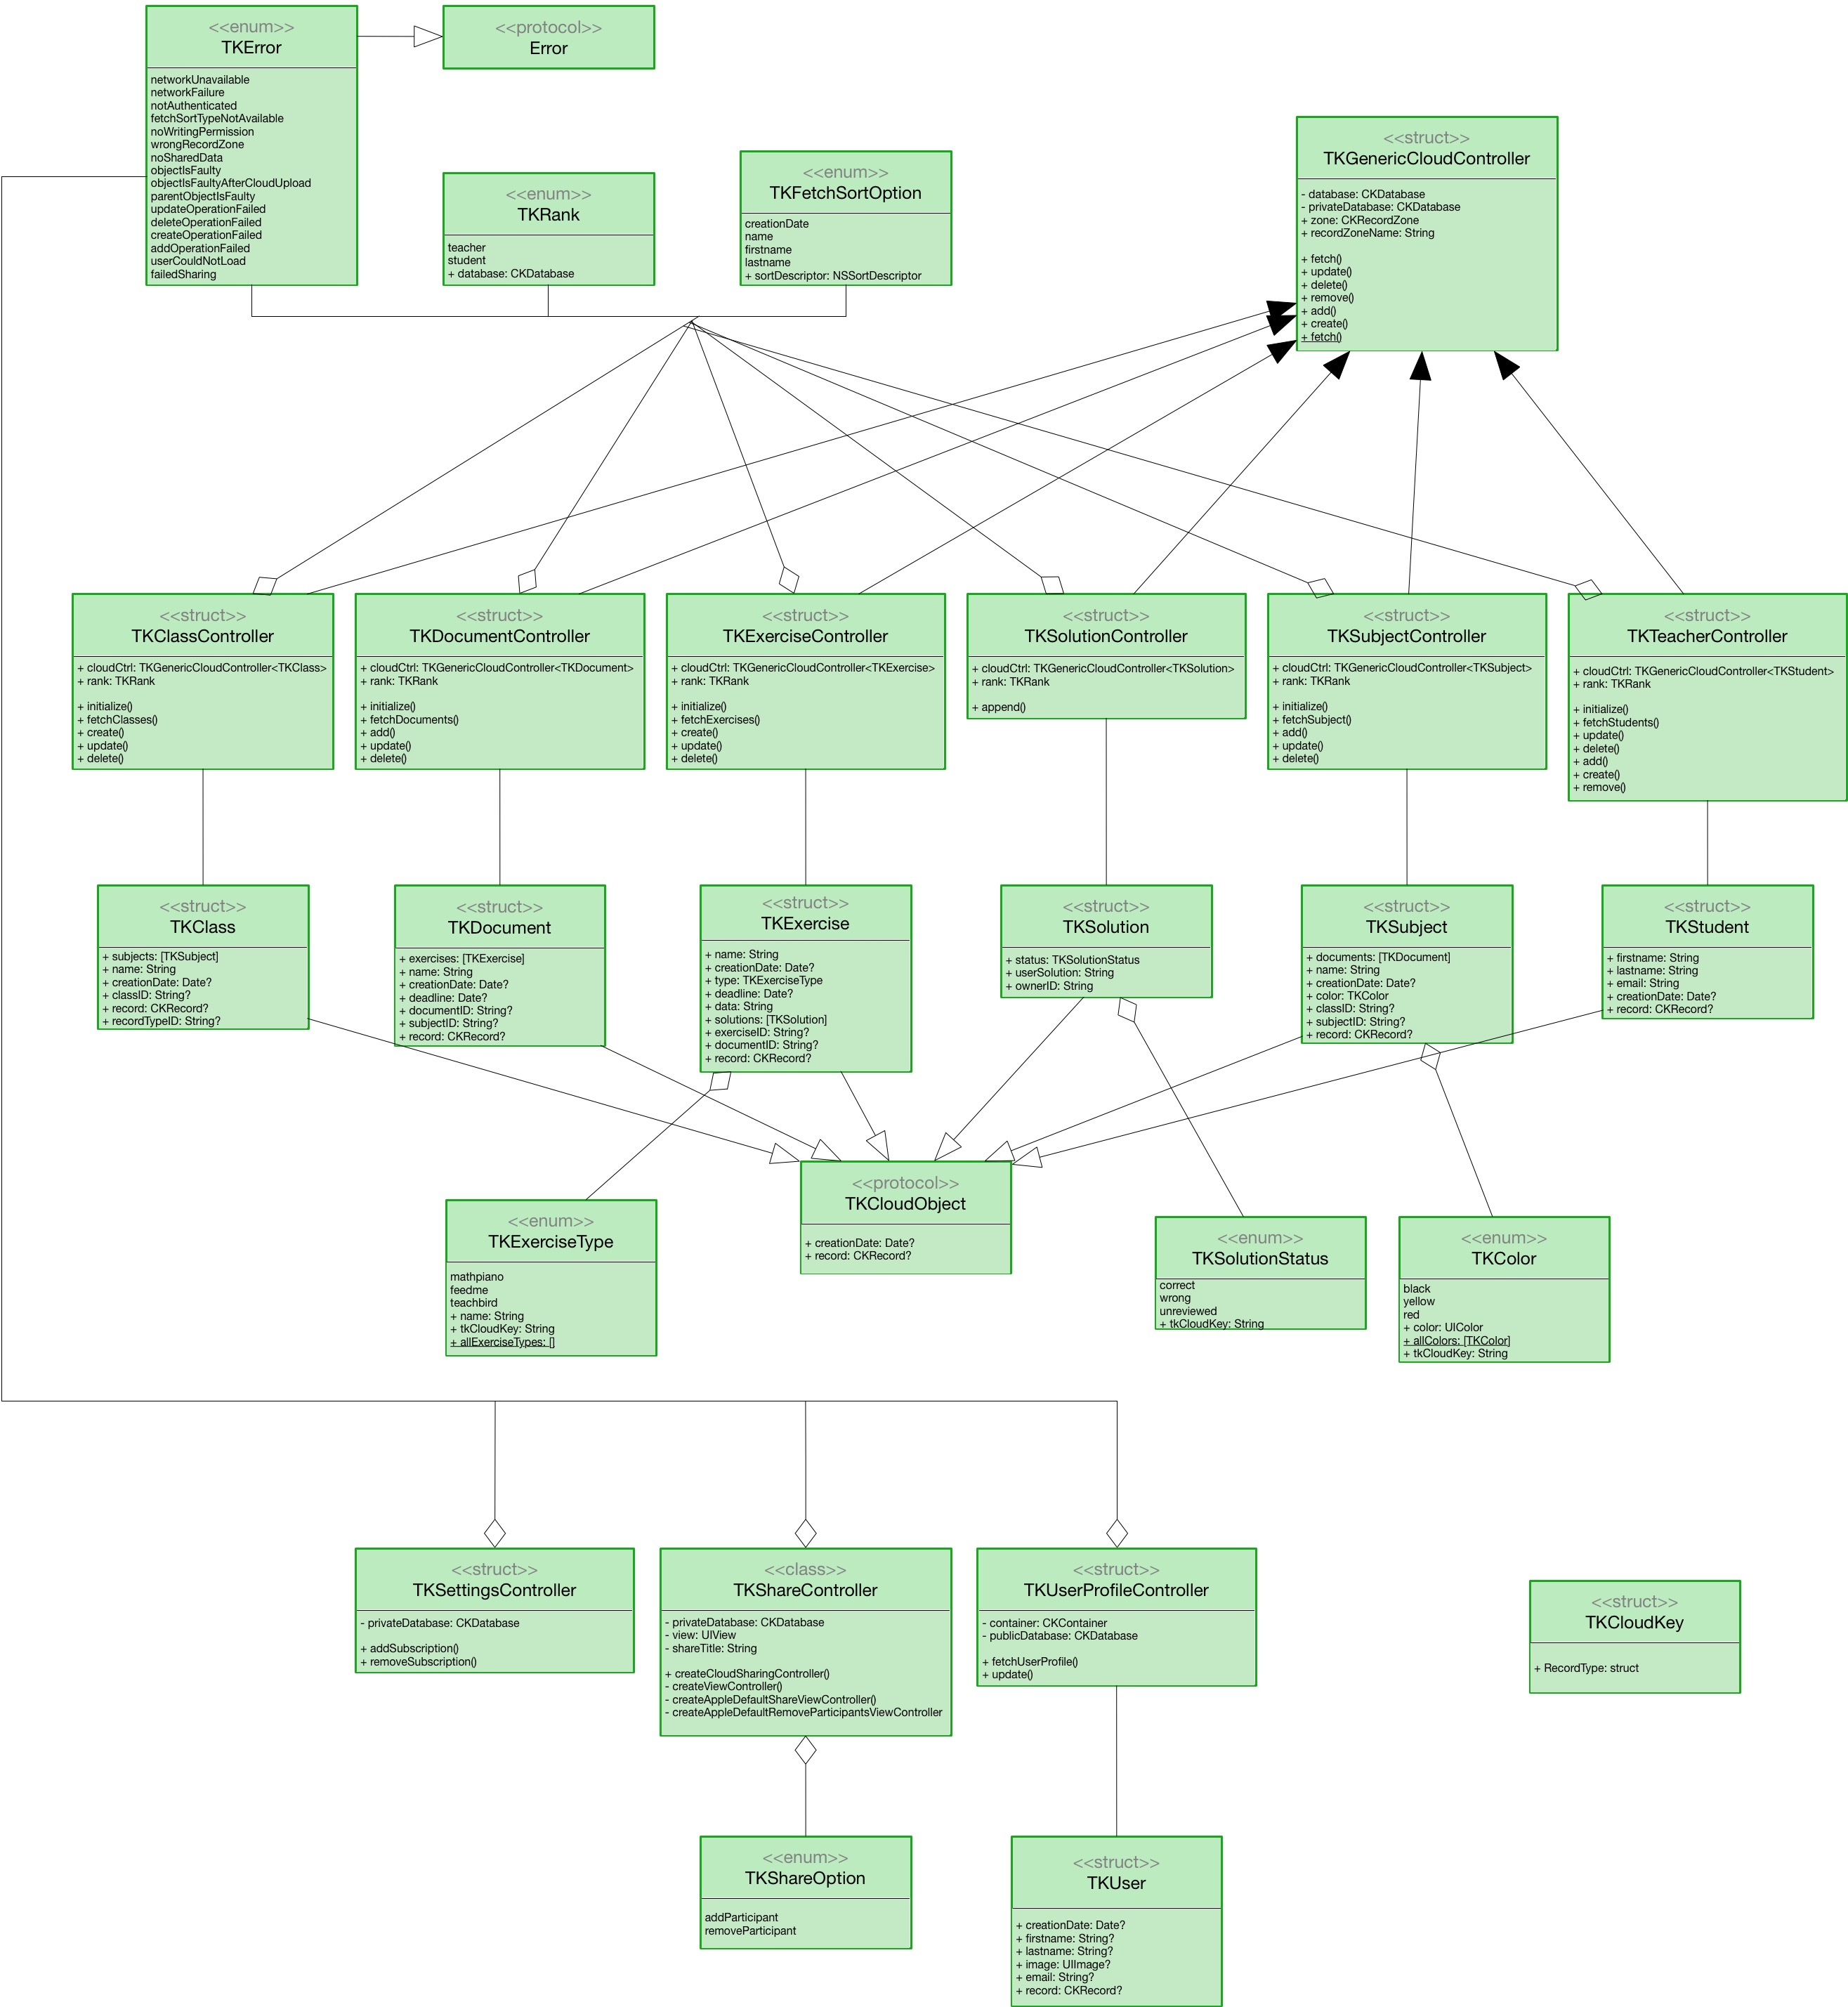
\includegraphics[width=\linewidth]{images/Klassendiagram_TeachKit.jpg}
  \caption{TeachKit Schnittstellen Klassendiagramm}
  \label{fig:diagramTeachKit}
\end{figure}

Auch TeachKit ist strikt nach der Model-View-Controller - Architektur aufgebaut. Hierbei erben alle Models, die in der Cloud gespeichert werden, von ihrer Superklasse TKCloudObject. Die Controller die diese Models verwalten, sind mit Hilfe eines generischen Controllers TKGenericCloudController implementiert worden. Alle Cloud-Models und Controller bedienen sich von verschiedenen Enumerations, die die Funktionalität übersichtlicher gestalten.

\newpage


\section{Features}

\subsection{Upload/Download/Delete/Fetch/Update}

Für jeden Datentyp in TeachKit, gibt es einen Controller der für die Operationen auf den Datentyp verantwortlich ist.
Somit gibt es folgende Controller für die Datentypen:

\begin{itemize}

\item TKClassController
\item TKSubjectController
\item TKDocumentController
\item TKExerciseController
\item TKSolutionController

\end{itemize}

Alle Controller sind ähnlich aufgebaut. Der Grund weshalb der Controller über die Methode initialize(…) funktionsfähig gemacht werden muss ist der, dass der Student auf die Shared-Database zugreift und diese zuerst gefetched werden muss.

Um doppelten Code zu vermeiden, arbeiten alle der oben genannten Controller mit dem TKGenericCloudController, der die Grundfunktionen übernimmt und in den jeweiligen Controllern dann spezialisiert werden.

\subsection{User Profile}

Zu jedem Nutzer kann der Vorname, Nachname und ein Profilbild gespeichert werden. Der TKUserProfileController der für die Nutzerverwaltung verantwortlich ist, arbeitet auf der Public-Database. Das bedeutet, dass alle Nutzer diese Informationen sehen können. Die aktuelle implementation erlaubt nur den download der Daten für den derzeit eingeloggten Nutzer. Diese kann erweitert werden, hätte aber momentan keine Verwendung gefunden.

\newpage

\subsection{Sharing}

Eines der wichtigsten Features unserer App ist das Teilen von Daten zwischen Teacher und Student. Nach dem Teilen gemeinsamer Daten haben beide Zugriff auf das Subject und alles was darunter angelegt ist.

CloudKit arbeitet mit drei verschiedenen Datenbanken.


\textbf{Private-Database}
\newline
Der aktuell angemeldete Nutzer ist der Inhaber der Daten, nur dieser hat Zugriff auf diese Datenbank und hat das Recht zu lesen und zu schreiben.
\newline
\textbf{Shared-Database}
\newline
Der aktuelle Nutzer ist nicht der Besitzer der geteilten Daten, und hat die beim Teilen zugewiesenen lese und/oder schreib Rechte.
\newline
\textbf{Public-Database}
\newline
Der aktuelle Nutzer ist nicht der Besitzer der geteilten Daten, und hat die beim Teilen Jeder App Nutzer hat lese Recht auf diese Daten, auch ohne aktiven iCloud Account.
\newline

Legt der Teacher seine Daten an, befinden diese sich in seiner private-Database. Nachdem dieser das Subject geteilt hat, befindet sich dies immer noch in der private-Database. Bei jedem Student der nun berechtigt ist, das geteilte Subject einzusehen, wird eine Referenz in der shared-Database gespeichert. Diese Referenz zeigt auf die Daten des Teachers in der private-Database.

Der Teacher teilt mit dem Student ein Subject, damit der Student die neue Arbeitsblätter einsehen kann. Mit dem Student wird der Zugriff auf Class nicht geteilt, weil er diese Information nicht benötigt.

\begin{center}
   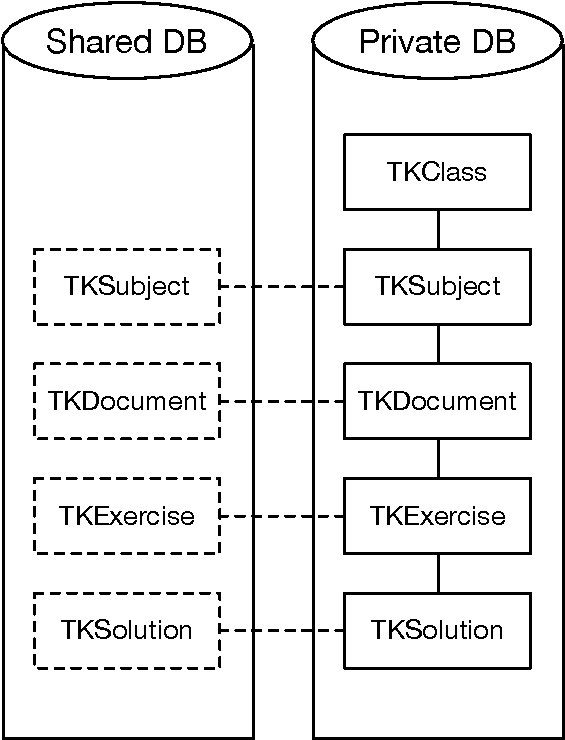
\includegraphics[width=5cm]{sharedDB_privateDB.pdf}
   \captionof{figure}{hared DB / Private DB}
\end{center}

Das Teilen findet über den TKShareController statt. Mit der Methode createCloudSharingController(…), wird der ViewController der für das Teilen verantwortlich ist erstellt und kann angezeigt werden.
Bei der Verwendung des Controllers müssen keine weiteren Bedingungen beachtet werden, der Controller kümmert sich um alles was zum Teilen benötigt wird.

\subsection{Push/Subscriptions}

Eine Besonderheit des CloudKits ist die einfache Implementierung von Push Benachrichtigungen bei Datenbankänderungen. PushNotifications in einer App zu implementieren, die über einen eigenen Server laufen, setzen PHP Kenntnisse voraus und können einiges an Zeit in Anspruch nehmen.
CloudKit Subscriptions sind jedoch einfacher zu implementieren und können auf Insert, Update, Delete und Create in der Datenbank reagieren.

Der Verwendungszweck der Subscriptions war dafür gedacht, dass der Student über Änderungen zu seinem Fach informiert wird. Dies könnte beispielsweise der Fall sein, wenn der Professor ein neues Arbeitsblatt seinem Fach hinzufügt.

Wir implementierten die CloudKit Subscriptions, die darauf reagiert, wenn der Teacher ein neues Document einem Subject hinzufügt.
Die ersten Tests auf zwei unterschiedlichen Geräten mit der gleichen Apple ID waren erfolgreich. Beim Testen über zwei unterschiedliche Apple ID’s, bei dem der Teacher ein Subject mit dem Student teilt, kamen wir allerdings an unsere Grenzen. Der Student wurde beim Hinzufügen eines neuen Objekts nicht benachrichtigt.
In der CloudKit API wurden wir dann auf die folgende Anmerkung aufmerksam, die besagt, dass Subscriptions auf der Shared-Database nicht unterstützt werden.

\newpage

\subsection{TKError}

Bei den meisten Aktionen die innerhalb des TeachKits Fehler auslösen können, werden Fehler vom Datentyp TKError erstellt. Jeder Fehler beinhaltet eine genauere Beschreibung des aufgetretene Problems. Folgende Fehler existieren:

\textbf{networkUnavailable}
Es besteht keine Internetverbindung.

\textbf{networkFailure}
Es besteht eine Internetverbindung, es konnte allerdings keine Verbindung zur Cloud hergestellt werden.

\textbf{wrongRecordZone}
Die Operation wird auf der falschen RecordZone ausgeführt oder existiert nicht. An Schnittstelle wenden.

\textbf{failedSharing}
Das Objekt konnte nicht geteilt werden.

\textbf{parentObjectIsFaulty}
Operation konnte nicht ausgeführt werden, da das Parent-Objekt Fehlerhaft ist.

\textbf{objectIsFaulty}
Operation konnte nicht ausgeführt werden, da das Objekt Fehlerhaft ist.

\textbf{objectIsFaultyAfterCloudUpload}
Auf dem Objekt wurde eine Operation in der Cloud ausgeführt. Das von der Cloud erhaltene Objekt ist inkonsistent.

\textbf{userCouldNotLoad}
Beim Zugriff auf die Nutzer Informationen ist ein Fehler unterlaufen.

\textbf{updateOperationFailed}
Der Datensatz konnte nicht geupdated werden.

\textbf{deleteOperationFailed}
Der Datensatz konnte nicht gelöscht werden.

\textbf{createOperationFailed}
Der Datensatz konnte nicht erstellt werden.

\textbf{addOperationFailed}
Der Datensatz konnte nicht hinzugefügt werden.

\textbf{fetchSortTypeNotAvailable}
Das Attribut nach dem sortiert werden soll existiert nicht.

\textbf{noWritePermission}
Der Nutzer hat keine Berechtigung die Daten zu ändern.

\textbf{noSharedData}
Die Operation konnte nicht ausgeführt werden, da noch keine Daten geteilt werden.

\newpage

\section{Aufgetretene Probleme}

\subsection{Subscription}
Da auf das Problem mit den Subscriptions bereits im Abschnitt Push/Subscriptions eingegangen wurde, erwähnen wir an dieser Stelle nur noch einmal, das Subscriptions nicht auf der Shared-Database unterstützt werden.


\subsection{Sharing}
Während der Implementation der Sharing Funktion, hatten wir über einen längeren Zeitraum das Problem, dass das Record zwischen den Nutzern geteilt wurde. Der darunter hängende Baum war allerdings nicht beim Student einzusehen.

\begin{center}
   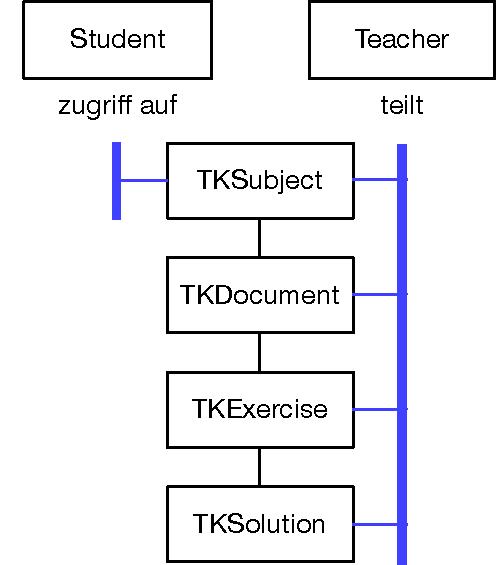
\includegraphics[width=5cm]{images/problemImage.pdf}
   \captionof{figure}{Zugriff Teacher/Student}
\end{center}

Letztendlich stellte sich heraus, dass die Verbindung zwischen Parent- und dem Child-Record nicht hergestellt wurde. Dieses Problem konnte ganz einfach mit der Methode setParent(CKRecord?) gelöst werden, allerdings musste man dafür erst wissen, dass so eine Funktion überhaupt existiert.

\newpage

\subsection{TKSolution}

Die Idee hinter TKSolution war die, dass ein Student seine Lösung darin erstellt und anschließend zu der TKExercise hinzufügt. Allerdings ist es dem Student nicht möglich, weitere Records in der geteilten Datenbank des Teachers zu erstellen und hinzuzufügen.

\begin{center}
   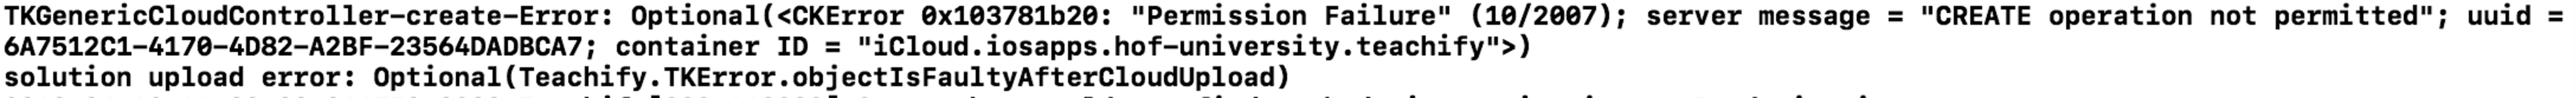
\includegraphics[width=15cm]{images/code_error.pdf}
   \captionof{figure}{Error}
\end{center}

Da diese Fehlermeldung auftritt obwohl wir die publicPermission des CKShare Objektes richtig gesetzt haben und immer noch kein Record erzeugen konnten, mussten wir eine andere Lösung dafür suchen. Wir entschlossen uns die Lösungen in ein Data-Objekt zu serialisieren und diese in TKExercise hinzuzufügen. 
Unseren neuen Lösungsansatz testen wir zuerst mit einem Attribut vom Datentyp String und nicht den eigentlich benötigten Datentyp Data. Beim ersten Upload in die iCloud werden die Records in der Cloud automatisch angelegt. Der erste Test hat geklappt und anschließend wollten wir unseren benötigten Daten vom Typ Data sichern. Da allerdings die angelegten Constraints nicht mehr für den neuen Datentyp gestimmt haben, konnten keine Records mehr hochgeladen werden. Die Constraints müssen zuerst im iCloud-Dashboard gelöscht und erneut hochgeladen werden.



%usw. ...


\listoffigures
\end{document}